\section{Performance Evaluation}
\label{sec:eval}

%Dynamic Datapath Configuration (DDC)
In this section, we will first demonstrate the benefits of \concept{} from two aspects: latency and total throughput, and then give the evaluation for the waypoints constraints computation part. All evaluations are run on an 3.5 GHz Intel i7 processor with 16 GB of RAM running Mac OSX 10.13.

\para{Methodology}: First we generate a random topology with 25 nodes and 50 edges. For every edge, we set two random values as its latency (5 - 10 ms) and bandwidth (5 - 10 Mbps). To model a flow in the topology, we randomly choose two nodes from the topology as the source and destination nodes of the flow. And a flow can have a sequence of nodes (other than its source and destination nodes) in the topology as its required ordered middleboxes for packet processing. (We add a constraint to the selection for these middlebox nodes that the number of neighbors of a middlebox node must equal to two as typically a middlebox does not have route selection capability, \ie, for any packet, it only has one output interface.) As a comparison of \concept{}, the traditional approach does not distinguish whether a middlebox is stateful or stateless. Therefore, when computing a path for a flow in the tradition way (\ie, do not apply \concept{}), it requires the path must pass through all the middleboxes in a correct order. And when computing a path for a flow in the \concept{} approach, we random choose a subset of its required middlebox nodes as stateful middleboxes since for \concept{} approach, stateful and stateless middleboxes are handled in different ways.

\para{Latency}: To show the benefits for the latency aspect, we consider a single flow and differentiate its number of required middleboxes. And the target is to find the optimal path to minimize the latency for the flow. Then, we compare the results (\ie, the minimal latency) between applying \concept{} and not.

\para{Total throughput}: To show the benefits for the total throughput aspect, we consider multiple flows and all flows have the same required middleboxes. We also differentiate the number of middleboxes. And the target is to find optimal paths that have maximum total throughput. Then, we compare the results (\ie, the maximum total throughput) between applying \concept{} and not.

\para{Execution time}: To evaluate the performance of \concept{}, we compare the execution time of the path computation to maximize total throughput for both approaches (\ie, applying \concept{} and not).

\para{Waypoints constraints computation}: To show the benefits of the waypoints constraints computation, we set a sequence of nodes in the topology as a flow's waypoints constraint. Then, we consider the minimal latency as system's objective and compare the results between applying the waypoints constraints computation and not (\ie, leading to excessive constraints). In the excessive constraints, all the middlebox nodes should be passed through before flow's waypoints.



\para{Results}: The results in Fig.~\ref{fig:eval12}(a) demonstrate that by using \concept{}, the latency can be reduced. Specifically, $F$ specifies the number of flows; $M$ specifies the number of required middleboxes for flows; $S$ specifies the number of stateful middleboxes for flows. As minimizing latency for a flow does not affect the results of other flows, the experiment only considers one flow scenario. From the results, we can see that without \concept{}, the latency of the flow grows up when the number of stateless middleboxes increases but if \concept{} is applied, the latency grows up only when the number of stateful middleboxes increases.

The results in Fig.~\ref{fig:eval12}(b) demonstrate that by using \concept{}, the total throughput can be increased. Specifically, when there are 5 flows and 3 middleboxes, the total throughput with \concept{} is around 3 times compared with that without \concept{}.

\begin{figure}[!htbp]
%\vspace{-2mm}
\centering
\begin{subfigure}{0.48\linewidth}
      \centering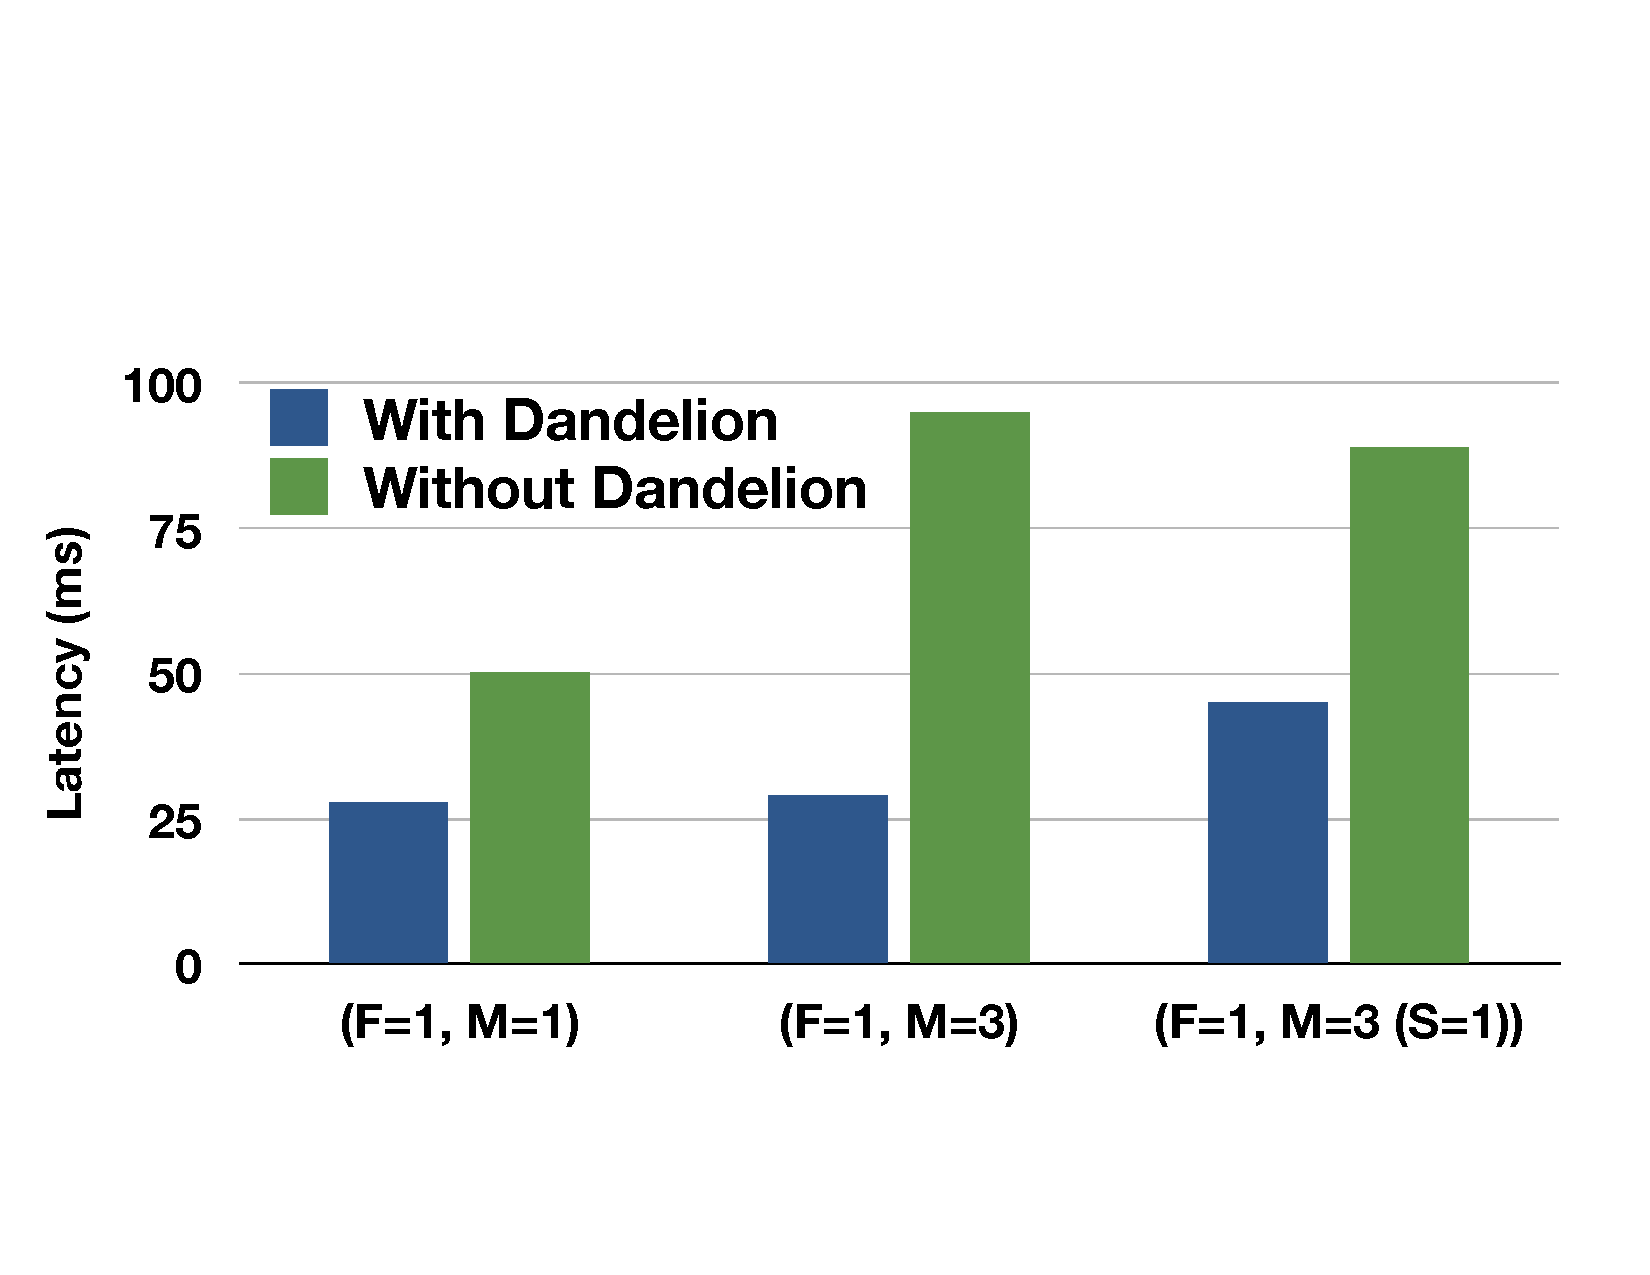
\includegraphics[width=\linewidth]{figures/ss-eval1.pdf}
      \caption{\label{fig:eval1} \small The latency for different scenarios.}
\end{subfigure}
%\hspace{0.03\linewidth}
\begin{subfigure}{0.48\linewidth}
      \centering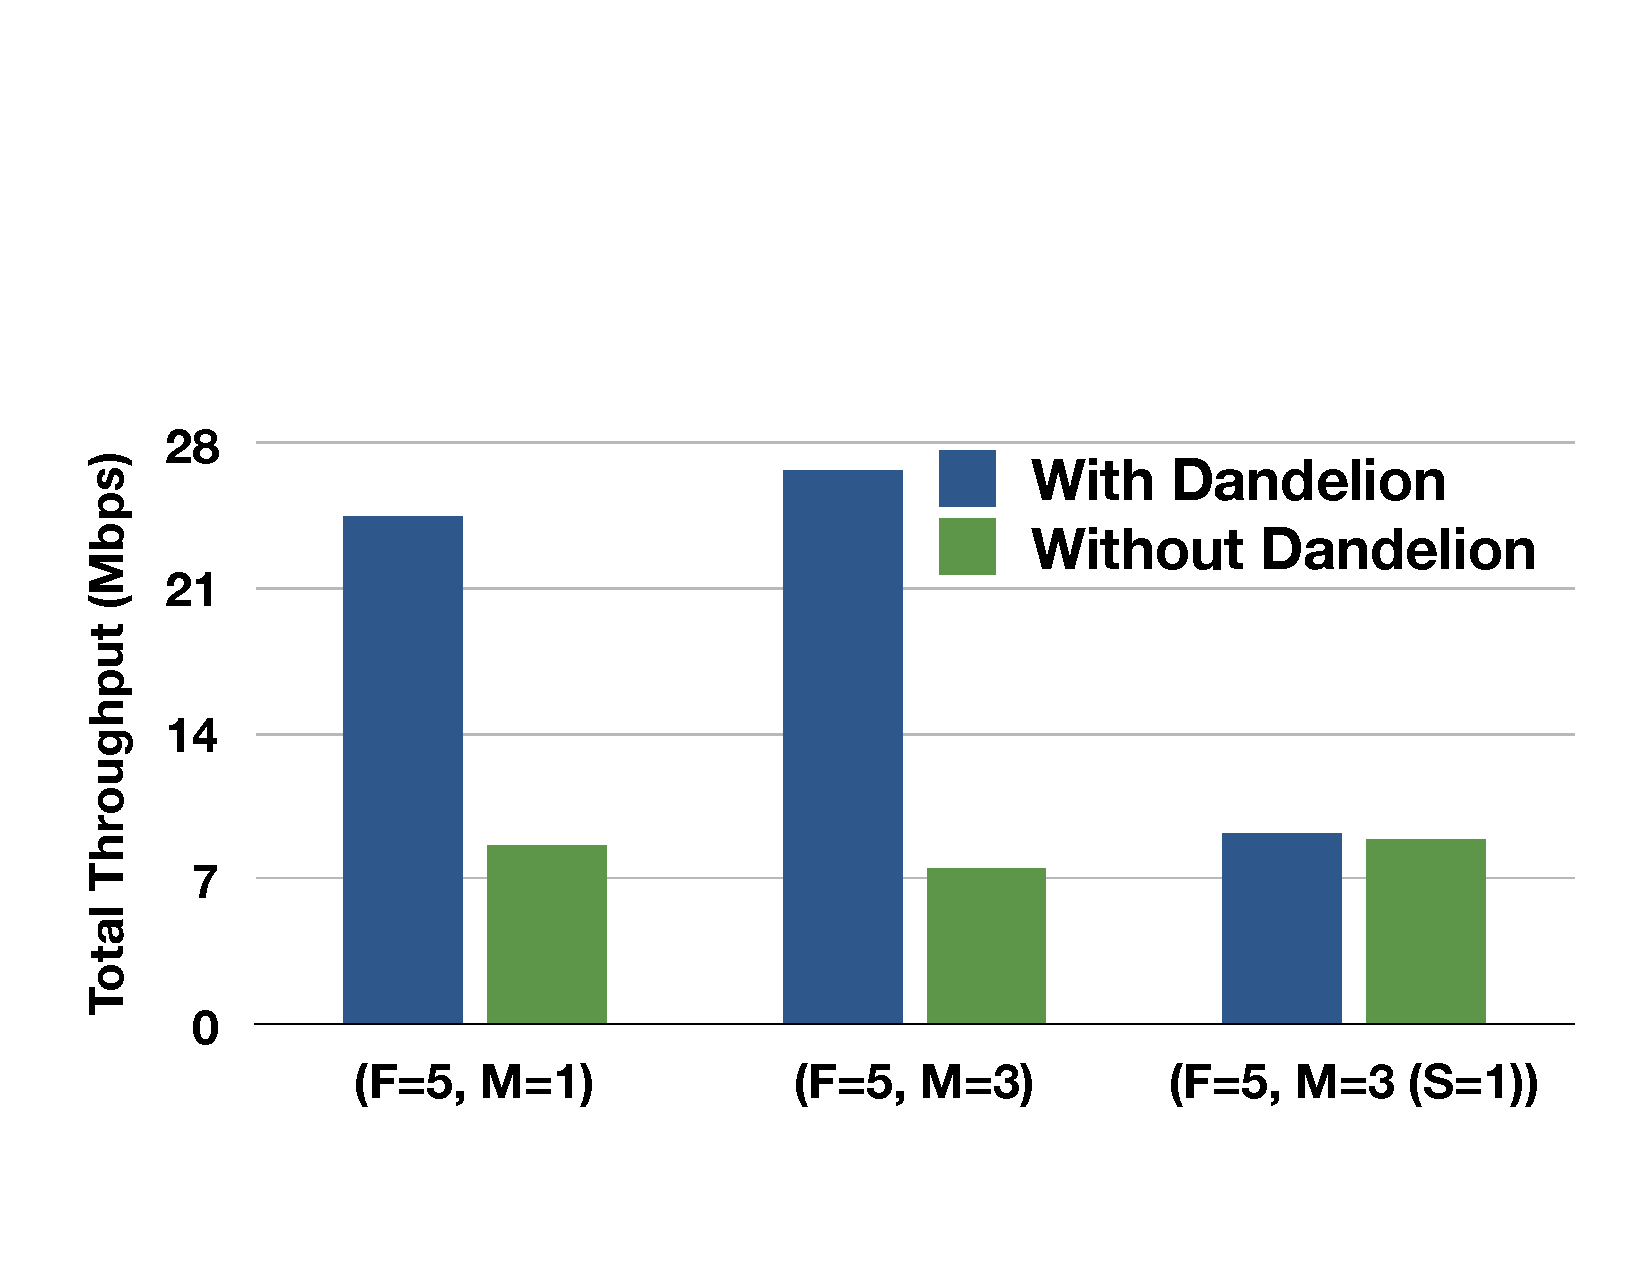
\includegraphics[width=\linewidth]{figures/ss-eval2.pdf}
      \caption{\label{fig:eval2} \small The total throughput for different scenarios.}
\end{subfigure}
\vspace{-2mm}
\caption{\small The benefits of \concept{} for latency and total throughput.}
%\vspace{-2mm}
\label{fig:eval12}
\end{figure}




%\begin{figure}[!htbp]
%%\vspace{-2mm}
%\centering
%\begin{subfigure}{0.8\linewidth}
%      \centering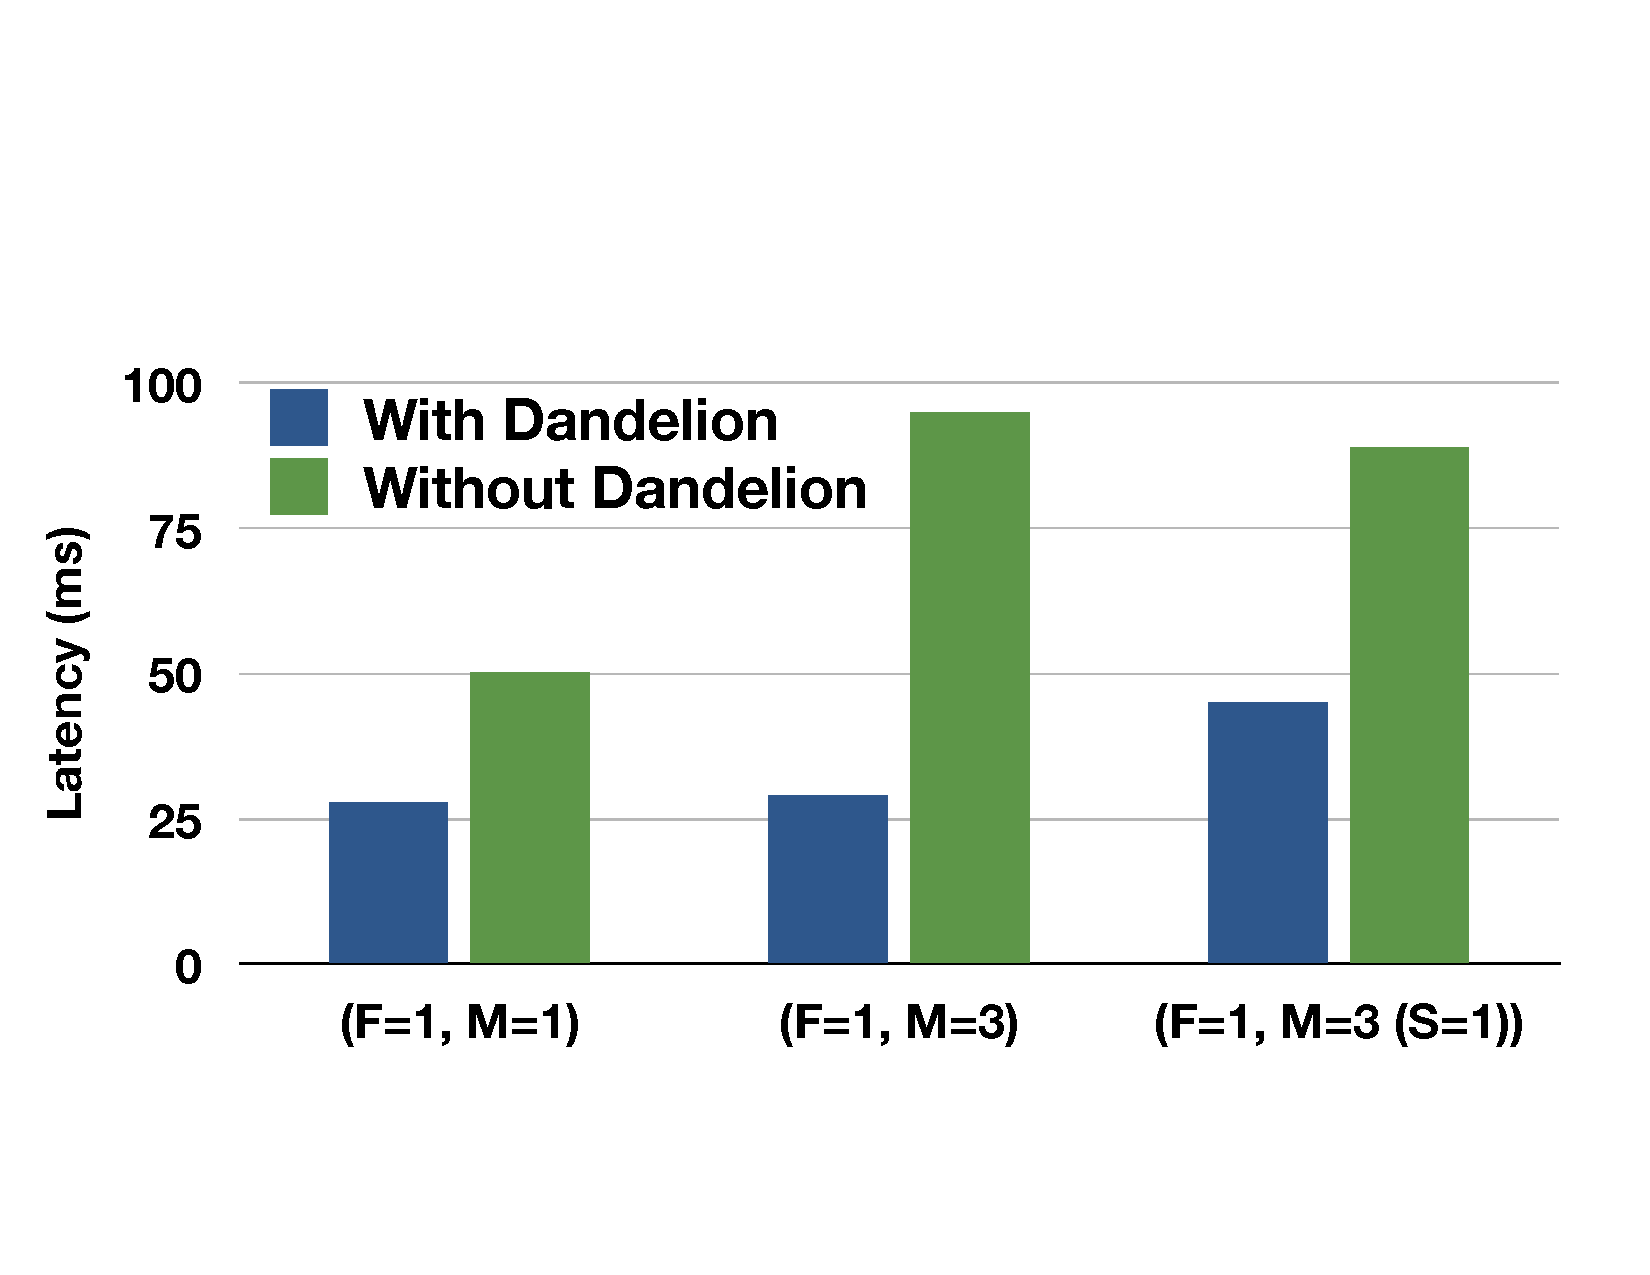
\includegraphics[width=\linewidth]{figures/ss-eval1.pdf}
%\end{subfigure}
%\hspace{0.03\linewidth}
%%\vspace{-2mm}
%%\caption{\footnotesize{The CDF of job latency local and remote jobs.}}
%\caption{\small The latency for different scenarios.}
%%\vspace{-2mm}
%\label{fig:eval1}
%\end{figure}




%\begin{figure}[!htbp]
%%\vspace{-2mm}
%\centering
%\begin{subfigure}{0.8\linewidth}
%      \centering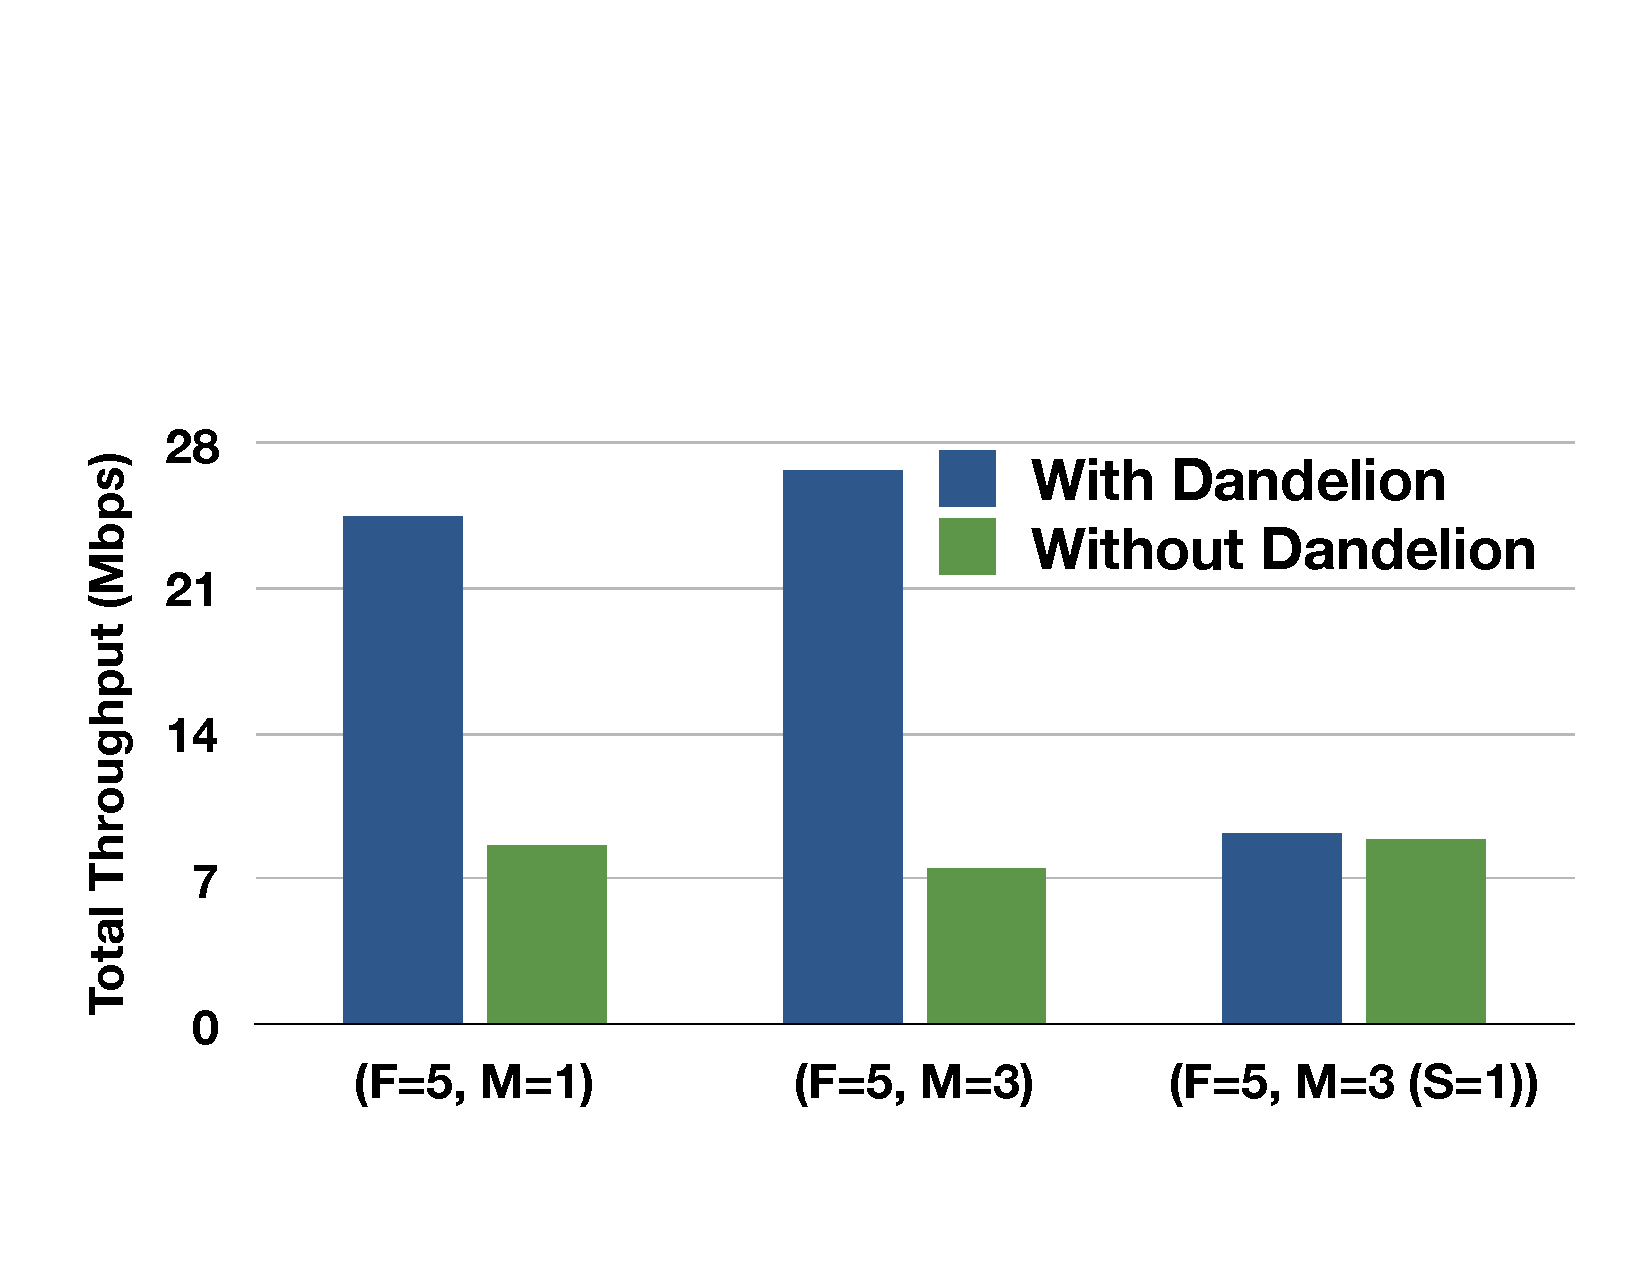
\includegraphics[width=\linewidth]{figures/ss-eval2.pdf}
%\end{subfigure}
%\hspace{0.03\linewidth}
%%\vspace{-2mm}
%%\caption{\footnotesize{The CDF of job latency local and remote jobs.}}
%\caption{\small The total throughput for different scenarios.}
%%\vspace{-2mm}
%\label{fig:eval2}
%\end{figure}

The results in Table~\ref{table:eval1} show the execution time of the path computation part to maximize total throughput. Since with \concept{}, the number of constraints is smaller than that without \concept{}, the execution time is also reduced (from 10.8 to 1.4 seconds when F=5 and M=3). 


\begin{table}[]
\footnotesize
\begin{tabular}{|l|l|l|l|}
\hline
             & \footnotesize(F=5, M=1) & \footnotesize (F=5, M=3) & \footnotesize (F=5, M=3 (S=1)) \\ \hline
With \concept{}    & 1.3 (s)    & 1.4 (s)    & 4.2 (s)          \\ \hline
Without \concept{} & 4.5 (s)    & 10.8 (s)   & 11.5 (s)         \\ \hline
\end{tabular}
\caption{\small The execution time of path computation to maximize total throughput for different scenarios.}
\label{table:eval1}
\end{table}


Fig.~\ref{fig:eval34} shows the latency with correct constraints (\ie, by
applying waypoints constraints computation) and with excessive constraints.
Specifically, the results in Fig.~\ref{fig:eval34}(a) consider that the
waypoints only have one node while Fig.~\ref{fig:eval34}(b) are for three nodes.
From the results, we can see the excessive constraints increase the latency,
\ie, lead to non-optimal path computation result. As the number of nodes
increases in the waypoints constraint, the latency with excessive constraints becomes larger.

\begin{figure}[!htbp]
%\vspace{-2mm}
\centering
\begin{subfigure}{0.48\linewidth}
      \centering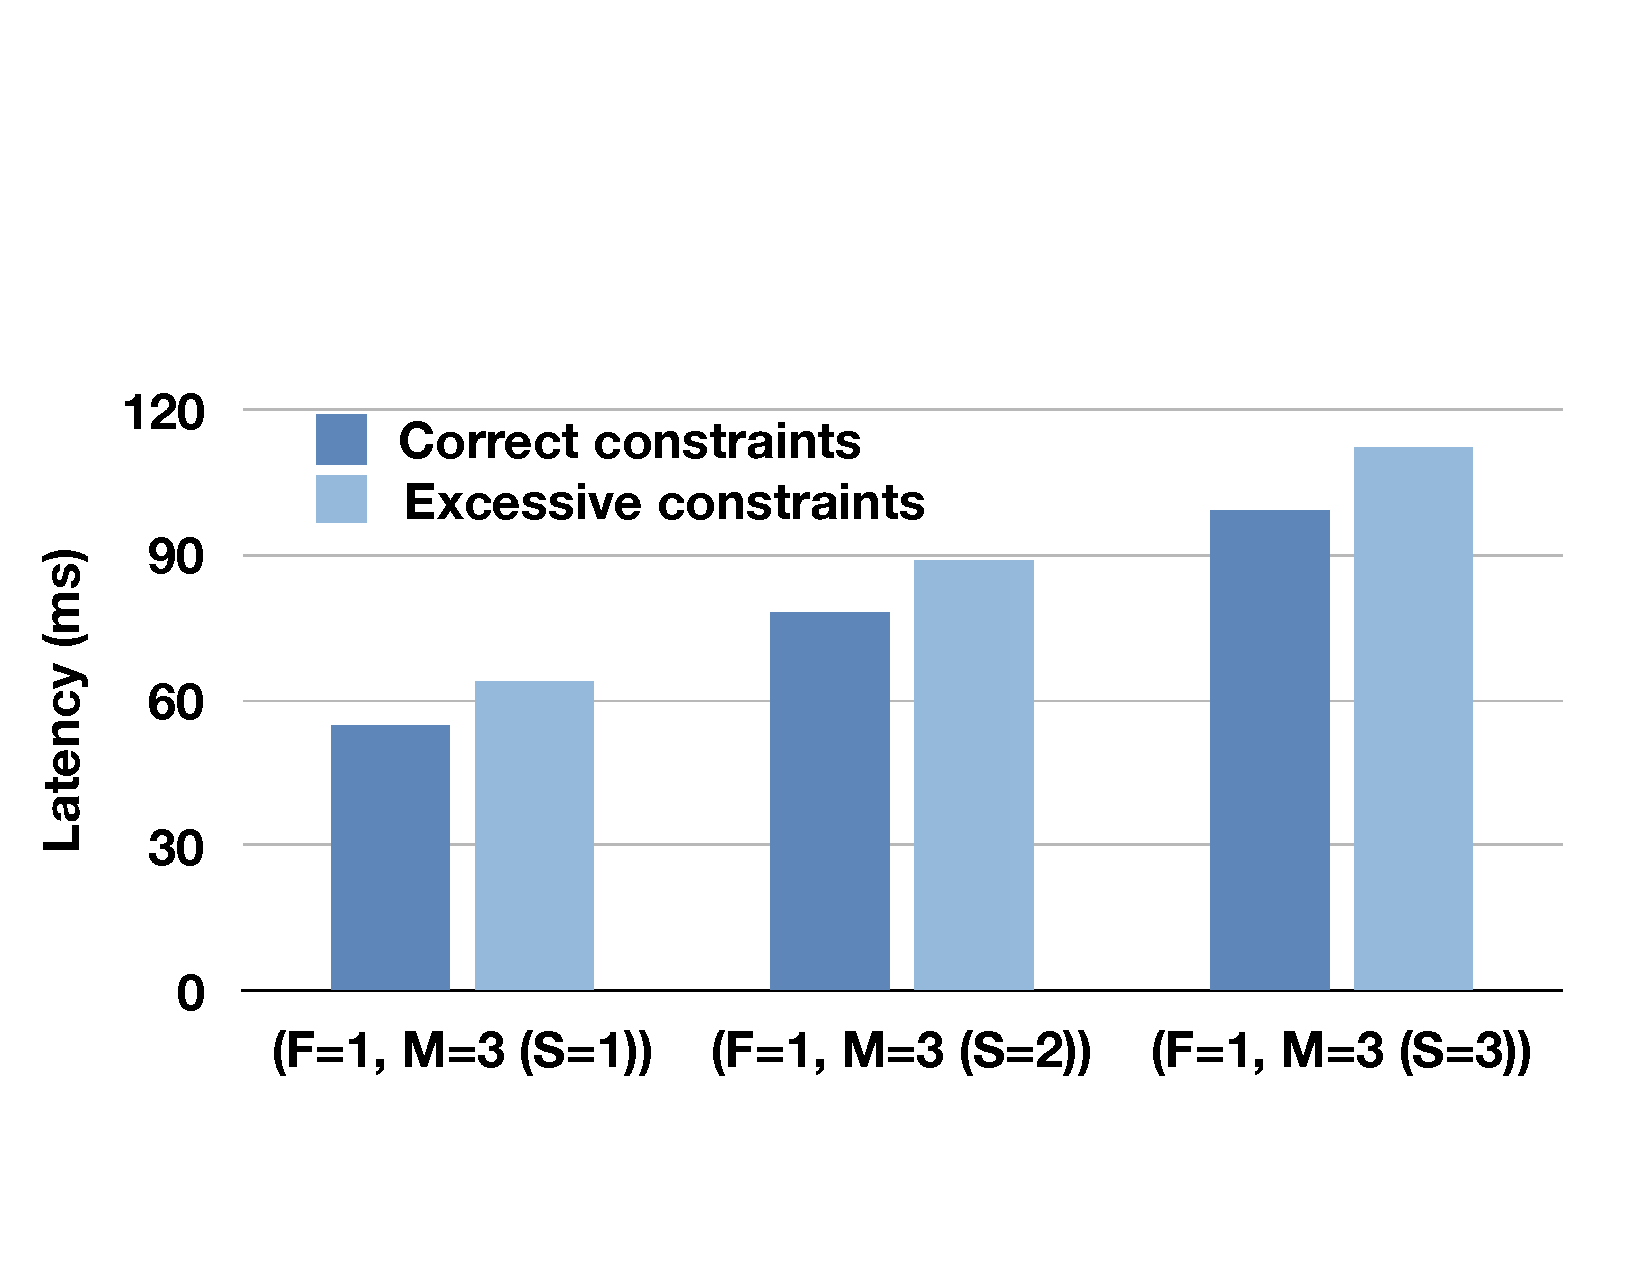
\includegraphics[width=\linewidth]{figures/ss-eval3.pdf}
      \caption{\label{fig:eval3} \small One node in waypoints constraint.}
\end{subfigure}
%\hspace{0.03\linewidth}
\begin{subfigure}{0.48\linewidth}
      \centering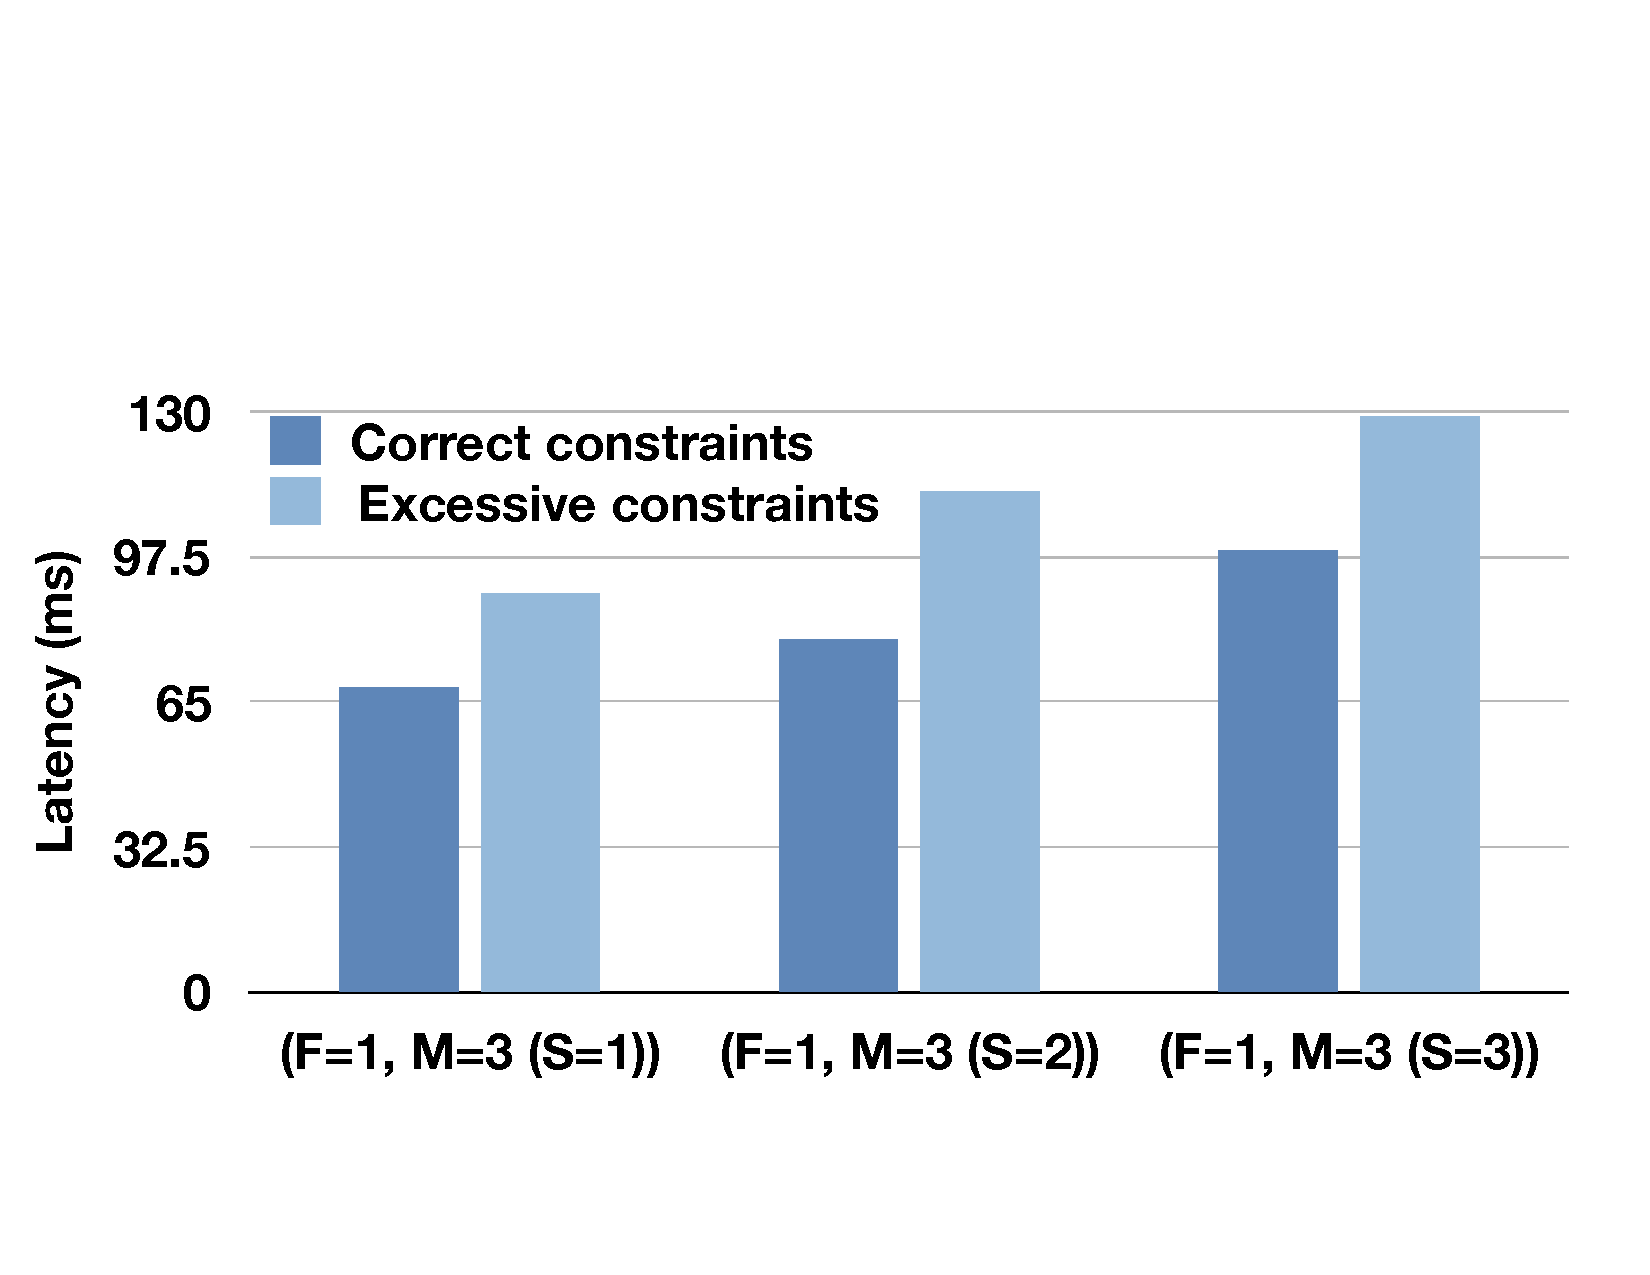
\includegraphics[width=\linewidth]{figures/ss-eval4.pdf}
      \caption{\label{fig:eval4} \small Three nodes in waypoints constraint.}
\end{subfigure}
\vspace{-2mm}
\caption{\small The latency with different waypoints constraints.}
%\vspace{-2mm}
\label{fig:eval34}
\end{figure}



%
%
%
%
%
%In this section, we will evaluate the proposed RSP design from two aspects: the execution time of pipeline design and the number of flow rules of the generated pipeline. All evaluations are run on an 3.5 GHz Intel i7 processor with 16 GB of RAM running Mac OSX 10.13.
%
%\subsection{Execution time}
%
%\para{Methodology}: Based on the analysis of the optimal pipeline design, we consider the following simple pipeline design algorithm: Given a DFG and $k$, recursively apply the source vertices selection $k-1$ times on the DFG to enumerates all the possible hardware pipelines. For the evaluation of both RSP and the unrolling approach, we randomly generate the DFG as the following: For the RSP, we change the number of software pipelines in the RSP (\ie, the number of iterations of the loop, $n$) and the number of vertices in the DFG of each pipeline (given the number of vertices, randomly generate the dataflow graph); For the unrolling approach, for each generated software pipeline in the RSP, we remove several vertices randomly. Then, we compare the execution time of RSP approach with the unrolling approach. Note that the complexity of enumerating all the possible pipelines equals to find the optimal pipeline as we do not consider the merging algorithm.
%
%%Then we evaluate the execution time of both RSP design and the unrolling approach. Specifically, for the evaluation of the RSP design, we change the number of software pipelines in the RSP and the number of vertices in the DFG of each pipeline (given the number of vertices, randomly generate the dataflow graph). To model the unrolling approach, for each pipeline in the repeated pipeline, we remove several vertices randomly. Then, we compare the execution time of repeated pipeline approach and the unrolling approach.
%
%\para{Result}: The result is shown in Figure~\ref{fig:eval1}. The horizontal axis specifies the number of iterations of the loop ($n$). The difference of Figure~\ref{fig:eval1-a} and Figure~\ref{fig:eval1-b} is the number of vertices ($m$) in the DFG of each software pipeline (for the unrolling approach, it means the number before removing vertices randomly) where $m = 10$ in Figure~\ref{fig:eval1-a} and $m = 20$ in Figure~\ref{fig:eval1-b}. And all the pipeline designs have the same $k$ as the limited number of flow tables where $k=10$. From the results, we can see that the RSP approach has smaller execution time compared (around 10 times when $n = 50$ and $m = 10$) with the unrolling approach when $k < n$. Note that when $n = 10$, both RSP and unrolling approach consider 10 software pipelines in the pipeline design, therefore, the execution time of both approaches is the same. And when $n = 100$, the execution time of unrolling is too large compared with the RSP approach.
%
%\begin{figure}[!htbp]
%%\vspace{-2mm}
%\centering
%\begin{subfigure}{0.47\linewidth}
%      \centering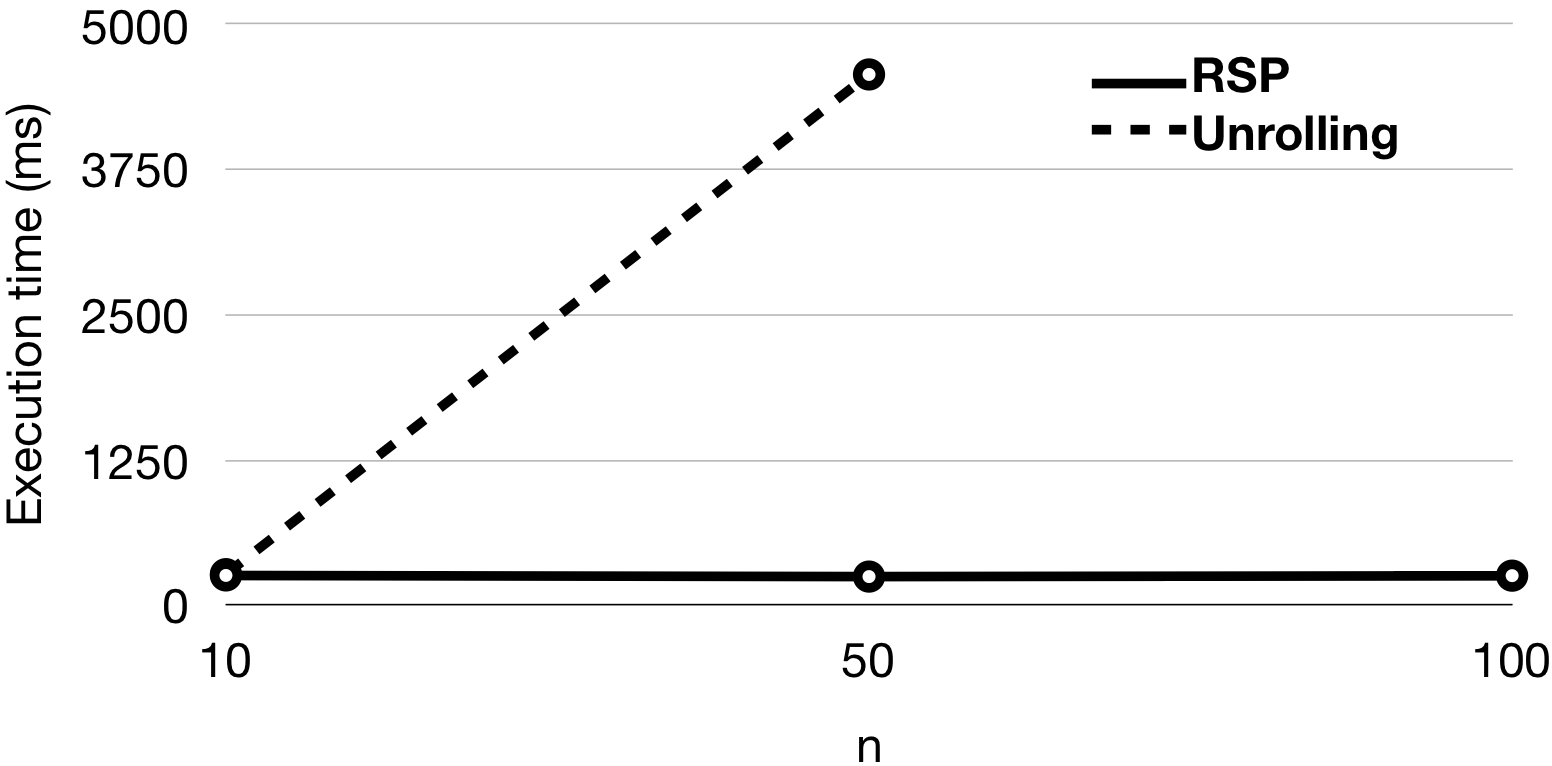
\includegraphics[width=\linewidth]{figures/lp-70.png}
%      \caption{\label{fig:eval1-a} \small $m$ = 10.}
%\end{subfigure}
%\hspace{0.03\linewidth}
%\begin{subfigure}{0.47\linewidth}
%      \centering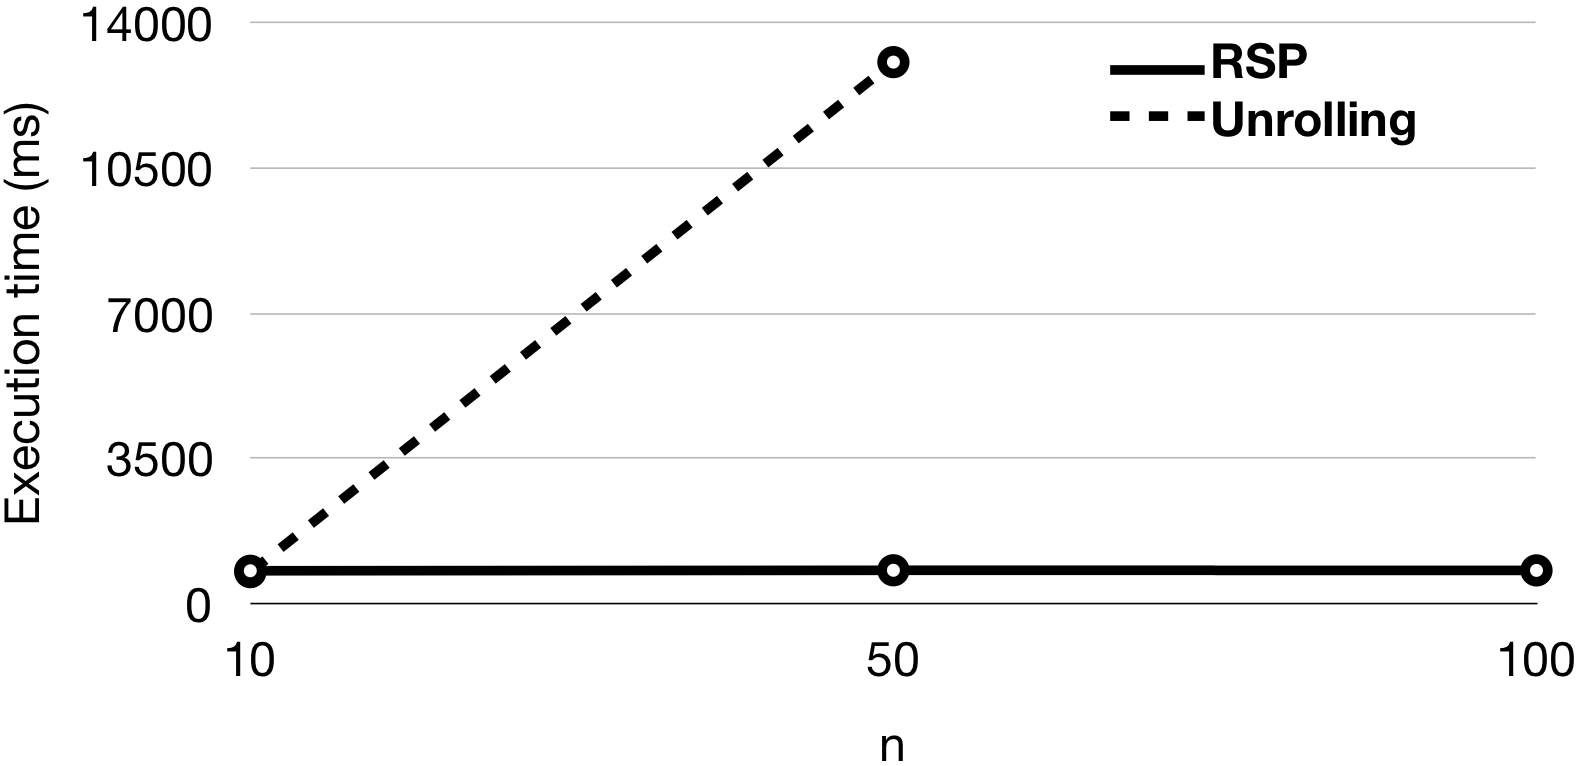
\includegraphics[width=\linewidth]{figures/lp-71.png}
%      \caption{\label{fig:eval1-b} \small $m$ = 20.}
%\end{subfigure}
%%\vspace{-2mm}
%%\caption{\footnotesize{The CDF of job latency local and remote jobs.}}
%\caption{\small The execution time of two approaches by changing the number of iterations ($n$) and the number of vertices ($m$).}
%%\vspace{-2mm}
%\label{fig:eval1}
%\end{figure}
%
%\subsection{Number of Flow Rules}
%
%\para{Methodology}: To compute the number of flow rules, we assign each variable (\ie, the vertex of DFG) the size of domain (\ie, the number of available values for the variable) randomly. Specifically, for the source vertices in the DFG of each software pipeline, we set the value from 100 to 200. And for the internal vertices in the DFG, we set the value from 10 to 20. This is because for the source vertices, they may represent packet fields which should have a larger range of values compared with internal variables in the program. Also, given a flow table, the computation of number of flow rules equals to the product of the size of domain of all the input variables. For example, a flow table consists of three input variables and their size of domain are 120, 10, 10 respectively, then the number of flow rules of the table is 12000. The definitions of $n$ and $m$ remain the same as the evaluation of execution time. We compare the number of flow rules of RSP design with the black-box approach (\ie, single table approach).
%
%\para{Result}: The result is shown in Table.~\ref{table:eval2}. As for the single table approach, the number of flow rules only depends on the first DFG of all software pipelines (which equals to the product of the size of domain of all the source vertices of the first DFG), so the values are the same for different $n$. From the result, we can find that the multi-table design can reduce the number of flow rules significantly compared with the single table approach. Also need to note that by the RSP approach, for each table, it may have a lot of unused flow rules. For example, the \codeword{while i in range(100)} statement can be viewed a flow table that matches \emph{i} and writes to \emph{i} with 100 flow rules (\ie, i = 0, 2, ..., 99), which has 99 unused flow rules when the table is the first table. Therefore, the number of flow rules can be reduced further by existing work which will not be discussed in this paper.
%
%\begin{table}[!htbp]
%\centering
%\begin{tabular}{|l|l|l|}
%\hline
%         & n =10, m = 10 & n = 50, m= 10 \\ \hline
%Single  & 3898434       & 3898434       \\ \hline
%RSP & 61856         & 224098        \\ \hline
%\end{tabular}
%\caption{\small The number of flow rules of the single table approach and the RSP approach.}
%\label{table:eval2}
%\end{table}
%

